%%%%%%%%%%%%%%%%%%%%%%%%%%%%%%%%%%%%%%%%%
% University Assignment Title Page 
% LaTeX Template
% Version 1.0 (27/12/12)
%
% This template has been downloaded from:
% http://www.LaTeXTemplates.com
%
% Original author:
% WikiBooks (http://en.wikibooks.org/wiki/LaTeX/Title_Creation)
%
% License:
% CC BY-NC-SA 3.0 (http://creativecommons.org/licenses/by-nc-sa/3.0/)
% 
% Instructions for using this template:
% This title page is capable of being compiled as is. This is not useful for 
% including it in another document. To do this, you have two options: 
%
% 1) Copy/paste everything between \begin{document} and \end{document} 
% starting at \begin{titlepage} and paste this into another LaTeX file where you 
% want your title page.
% OR
% 2) Remove everything outside the \begin{titlepage} and \end{titlepage} and 
% move this file to the same directory as the LaTeX file you wish to add it to. 
% Then add \input{./title_page_1.tex} to your LaTeX file where you want your
% title page.
%
%%%%%%%%%%%%%%%%%%%%%%%%%%%%%%%%%%%%%%%%%
%\title{Title page with logo}
%----------------------------------------------------------------------------------------
%	PACKAGES AND OTHER DOCUMENT CONFIGURATIONS
%----------------------------------------------------------------------------------------

\documentclass[12pt]{article}
\usepackage[english]{babel}
\usepackage[utf8x]{inputenc}
\usepackage{amsmath}
\usepackage{graphicx}
\usepackage[colorinlistoftodos]{todonotes}
\usepackage{subcaption}

\begin{document}

\begin{titlepage}

\newcommand{\HRule}{\rule{\linewidth}{0.5mm}} % Defines a new command for the horizontal lines, change thickness here

\center % Center everything on the page
 
%----------------------------------------------------------------------------------------
%	HEADING SECTIONS
%----------------------------------------------------------------------------------------

% Name of your university/college
\textsc{\LARGE Instituto Superior T\'{e}cnico}\\[1.5cm]
% Major heading such as course name
\textsc{\Large ISR}\\[0.5cm]
% First Minor heading such as course title
\textsc{\large Report}\\[0.25cm]
% Second Minor heading such as course title
\textsc{\small State Of The Art Milestone}\\[0.25cm]

%----------------------------------------------------------------------------------------
%	TITLE SECTION
%----------------------------------------------------------------------------------------

\HRule \\[0.5cm]
{ \large \bfseries State Of The Art Essay: A First Approach}\\[0.25cm] % Title of your document
\HRule \\[0.5cm]
 
%----------------------------------------------------------------------------------------
%	AUTHOR SECTION
%----------------------------------------------------------------------------------------

\begin{minipage}{0.4\textwidth}
\begin{flushleft} \large
\emph{Author:}\\
Francisco Maria \textsc{Calisto} % Your name
\end{flushleft}
\end{minipage}
~
\begin{minipage}{0.4\textwidth}
\begin{flushright} \large
\emph{Coordinator:} \\
Professor Jacinto \textsc{Peixoto} % Coordinator's Name
\end{flushright}
~
\begin{flushright} \large
\emph{Co-Coordinator:} \\
Professor Daniel \textsc{Gon\c{c}alves} % Co-Coordinator's Name
\end{flushright}
\end{minipage}\\[2cm]

% If you don't want a supervisor, uncomment the two lines below and remove the section above
%\Large \emph{Author:}\\
%John \textsc{Smith}\\[3cm] % Your name

%----------------------------------------------------------------------------------------
%	DATE SECTION
%----------------------------------------------------------------------------------------

{\large 07/03/2016}\\[1cm] % Date, change the \today to a set date if you want to be precise

%----------------------------------------------------------------------------------------
%	LOGO SECTION
%----------------------------------------------------------------------------------------


\includegraphics{ist-logo.png}\\[0.5cm] % Include a department/university logo - this will require the graphicx package


\includegraphics{isr-logo.png}\\[0.5cm] % Include a department/university logo - this will require the graphicx package
 
%----------------------------------------------------------------------------------------

\vfill % Fill the rest of the page with whitespace

\end{titlepage}

\section{Introduction}

The Medical Imaging Multimodality Breast Cancer Diagnosis is a topic of great interest, it has been the subject of much work in the world of medicine, but few developments in terms of innovation in the computational world. An Application like this has a wide spectrum fields reference from surveillance based systems to medical application.

A vast majority of masses and calcifications can be accurately diagnosed from cytological features [1] of the cells that constitute them. However, the diagnostic accuracy depends on the training, experience, and many indefinite factors of interpretation of the medical expert in cytological evaluation.

There was, in fact, some developments in the past facing the classification system Computer-Based [2, 3] that assists in the diagnosis of breast cells based on visual assessment of characteristics of the cells. [4] A set of cytologic features, previously evaluated visually, are now replaced by digital ones, evaluated by image analysis. In this project we will compare the human precision in cytological diagnosis of breast cancer by digital image analysis accuracy combined with Computer-Based Machine Learn classification.

\section{User Interface Contextualisation}

The first step in successfully analysing the digital image is to specify the exact location of each masses nucleus or calcifications nucleus. The image is projected onto a computer screen, and the clinical medical operator uses, preferentially, a mouse button that will trace a rough outline of each visible masses (Figure 1) nucleus. On the other hand, the clinical medical operator will mark with dots the calcification (Figure 2) nucleus of cells.

% Commands to include a figure:
\begin{figure}[!hbt]
\centering
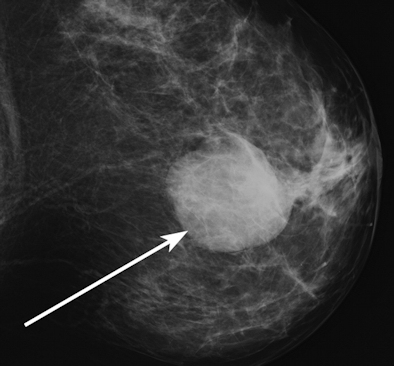
\includegraphics[width=0.75\textwidth]{masses.png}
\caption{\label{fig:frog}Mammographic image of a high-density mass (arrow)
}
\end{figure}

% Commands to include a figure:
\begin{figure}[!hbt]
\centering
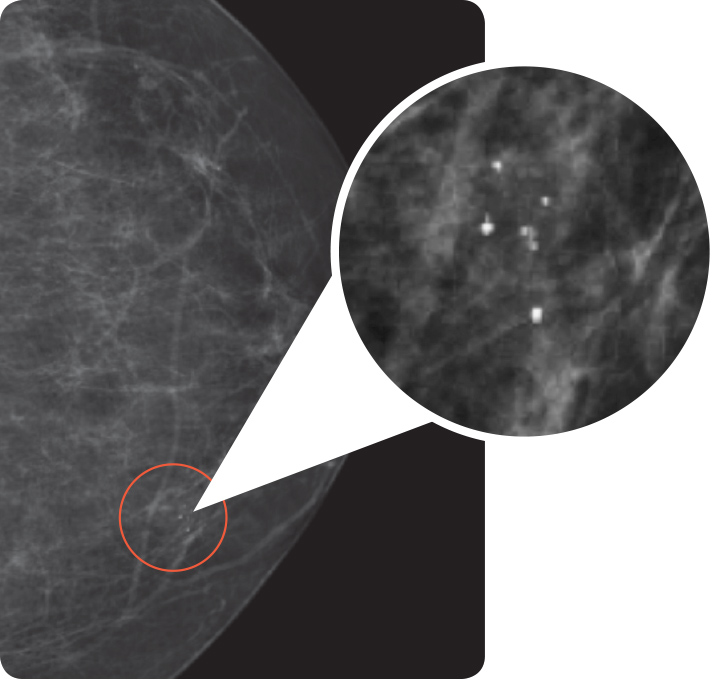
\includegraphics[width=0.75\textwidth]{calcifications.png}
\caption{\label{fig:frog}Mammogram – shows calcifications, an early sign of breast cancer
}
\end{figure}

\clearpage

\begin{thebibliography}{}
\bibitem{} William H. Wolberg, W. Nick Street, Olvi L. Mangasarian. Breast Cytology Diagnosis. \emph{Via Digital Image Analysis}, 1993.
\bibitem{} Bennett KP, Mangasarian OL. Robust linear programming discrimination of two linearly inseparable sets. \emph{Optimization Methods and Software 1:23-34}, 1992.
\bibitem{} Mangasarian OL. Multi-surface method of pattern separation. \emph{IEEE Transactions on Information Theory IT-14:801-807}, 1968.
\bibitem{} Wolberg WH, Mangasarian OL. Multisurface method of pattern separation for medical diagnosis applied to breast cytology. \emph{Proceedings of the National Academy of Sciences, U.S.A. 87:9193-9196}, 1992.
\end{thebibliography}

\end{document}
